\section{Expérimentation}
\begin{frame}{Description de l'expérimentation}
\begin{figure}
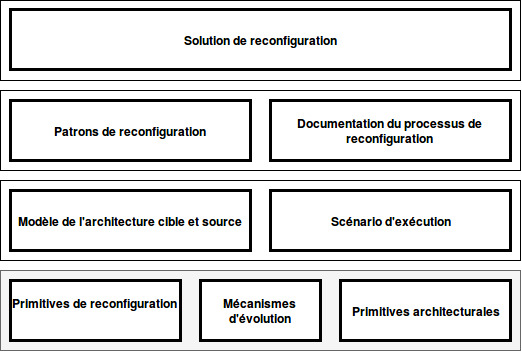
\includegraphics[width=0.7\textwidth]{imgs/framework}
\caption{\underline{\textbf{Framework de reconfiguration}}}
\end{figure}    
\end{frame}

%\begin{frame}{Itérations}
%\end{frame}

\begin{frame}{Interprétation et limite sur la réutilisation des
patrons de reconfiguration}
Résolution réconfiguration 
\begin{itemize}
\item 3 itérations
\item utilisation : co-évolution et tranquilité
\end{itemize}

L'architecte a pu :
\begin{itemize}
\item envisager plusieurs solutions
\item être aidé dans ses choix de solution
\item mettre en \oe{}vre la solution
\end{itemize}

limites : 
\begin{itemize}
\item sujets sont partis pris dans la conception des patrons
\item scénario de test simplifié
\end{itemize}

\end{frame}
